% -------------------------------------------------
% Fifteen-frame academic presentation
% Source: Radiuk_AuditablePost-hocECG_revised.docm
% Template: 85_Pres_v0.2.zip (KhNU Beamer theme)
% -------------------------------------------------

\documentclass[aspectratio=169,xcolor=dvipsnames]{beamer}
\usetheme{KhNU}

\usepackage[T1]{fontenc}
\usepackage[utf8]{inputenc}
\usepackage{amsmath}
\usepackage{amssymb}
\usepackage{array}
\usepackage{booktabs}
\usepackage{graphicx}
\usepackage{tabularx}
\usepackage{tikz}
\usetikzlibrary{calc,positioning}

\hypersetup{
  colorlinks=true,
  linkcolor=dexpiBlue,
  urlcolor=dexpiBlue
}

\setbeamertemplate{caption}{\raggedright\insertcaption\par}
\setlength{\tabcolsep}{3pt}
\renewcommand{\arraystretch}{1.12}
\newcolumntype{Y}{>{\raggedright\arraybackslash}X}
\newcolumntype{L}[1]{>{\raggedright\arraybackslash}p{#1}}
\newcolumntype{C}[1]{>{\centering\arraybackslash}p{#1}}

\setbeamercolor{equation box}{fg=dexpiBlueDark,bg=dexpiBlueLight}
\setbeamercolor{metric box}{fg=dexpiGreenDark,bg=dexpiGreenLight}

\newcommand{\compactitem}{\setlength{\itemsep}{0.28em}\setlength{\parskip}{0pt}}
\newcommand{\slidecaption}[1]{\par\vspace{0.08em}{\scriptsize\raggedright #1\par}}
\newcommand{\metric}[1]{%
  \begin{beamercolorbox}[wd=\linewidth,sep=0.45em,center]{metric box}%
    {\small\bfseries #1\par}%
  \end{beamercolorbox}%
}

% Supporting organizations represented in the supplied template and workspace.
% logo_ceur.svg is the vector duplicate of logo_ceur.png; the PNG is used for
% portable pdfLaTeX/Tectonic compilation.
\newcommand{\supportlogos}{%
  
\includegraphics[height=0.65cm]{assets_ecg/logo_ceur.png}\hspace{0.44cm}%
  
\includegraphics[height=0.65cm]{assets_ecg/logo_cs.png}\hspace{0.44cm}%
  
\includegraphics[height=0.65cm]{assets_ecg/logo_khmnu.png}\hspace{0.44cm}%
  
\includegraphics[height=0.65cm]{assets_ecg/logo_knu.png}\hspace{0.44cm}%
  
\includegraphics[height=0.65cm]{assets_ecg/logo_warwick.png}\hspace{0.44cm}%
  
\includegraphics[height=0.65cm]{assets_ecg/logo_xai.png}%
}

% Required PROFIT logo: top-right on every titled frame, never on title frame.
\addtobeamertemplate{frametitle}{}{%
  \begin{tikzpicture}[remember picture,overlay]
    \node[anchor=north east,inner sep=0pt]
      at ([xshift=-0.32cm,yshift=-0.13cm]current page.north east)
      {
\includegraphics[width=2.15cm]{assets_ecg/logo_profit.png}};
  \end{tikzpicture}%
}

\title{\Large\texorpdfstring{\textbf{Auditable Post-hoc ECG Explainability by Global\\Semantic Transition and Rough-Set Rules}}{Auditable Post-hoc ECG Explainability by Global Semantic Transition and Rough-Set Rules}}
\subtitle{\small A model-agnostic audit layer for frozen deep ECG classifiers}
\author{\small Pavlo Radiuk\textsuperscript{1} \and Oleksander Barmak\textsuperscript{1} \and Iurii Krak\textsuperscript{2,3}}
\institute{\scriptsize
  \textsuperscript{1}Khmelnytskyi National University\\
  \textsuperscript{2}Taras Shevchenko National University of Kyiv\\
  \textsuperscript{3}V.M. Glushkov Institute of Cybernetics
}
\date{\scriptsize 2026}

\begin{document}

% 1 -----------------------------------------------
\begin{frame}[plain]
  \titlepage
\end{frame}

\section{Motivation}

% 2 -----------------------------------------------
\begin{frame}{Clinical Need and Contributions}
\small
\begin{columns}[T,onlytextwidth]
  \column{0.31\textwidth}
  \begin{alertblock}{Audit gap}
  \small
  Accurate ECG classifiers rarely expose whether a decision used RR irregularity,
  QRS widening, QTc prolongation, or lead quality.
  \end{alertblock}

  \column{0.31\textwidth}
  \begin{block}{Post-hoc bridge}
  \small
  A regularized operator maps frozen 512-dimensional latent vectors to 43
  clinician-facing measurements.
  \end{block}

  \column{0.31\textwidth}
  \begin{exampleblock}{Symbolic audit}
  \small
  WEDD states and rough-set rules expose support, confidence, conflict,
  abstention, and predicate alignment.
  \end{exampleblock}
\end{columns}
\vspace{0.35em}
\begin{beamercolorbox}[wd=\linewidth,sep=0.55em]{equation box}
{\small\centering
\textbf{Frozen classifier} $\rightarrow$ semantic reconstruction $\rightarrow$
stable predicates $\rightarrow$ auditable rulebook $\rightarrow$ clinical review
\par}
\end{beamercolorbox}
\vfill
{\scriptsize
Research question: how much black-box behavior can be translated into explicit,
verifiable ECG logic without retraining the primary classifier?
\par}
\end{frame}

\section{Background}

% 3 -----------------------------------------------
\begin{frame}{Positioning Against Explanation Families}
\scriptsize
{\scriptsize\textbf{Table 6.} Quantitative comparison with representative
state-of-the-art explanation families.\par}
\vspace{0.18em}
\begin{tabularx}{\linewidth}{Ycccccc}
\toprule
\textbf{Approach} & \textbf{Post-hoc} & \textbf{Predicates} &
\textbf{Rule coverage} & \textbf{Conflict log} &
\textbf{Abstention log} & \textbf{Retraining}\\
\midrule
Saliency / attribution (Salih et al., 2024) & yes & no & 0.000 & no & no & no\\
TCAV (Kim et al., 2018) & yes & yes & 0.000 & no & no & no\\
Interpretable-model view (Rudin et al., 2019) & no & yes & method-specific & method-specific & method-specific & yes\\
Transition matrix (Radiuk et al., 2024) & yes & yes & 0.000 & no & no & no\\
Rough-set DSS (Singh et al., 2024) & yes & yes & qualitative & yes & partial & no\\
Concept bottleneck (Koh et al., 2020) & no & yes & 0.000 & no & no & yes\\
\textbf{Proposed B1} & \textbf{yes} & \textbf{yes} & \textbf{0.939} &
\textbf{0.0707} & \textbf{0.061} & \textbf{no}\\
\textbf{Proposed B2} & \textbf{yes} & \textbf{yes} & \textbf{0.900} &
\textbf{0.0000} & \textbf{0.100} & \textbf{no}\\
\bottomrule
\end{tabularx}
\vspace{0.20em}
\begin{columns}[T,onlytextwidth]
  \column{0.48\textwidth}
  \begin{beamercolorbox}[wd=\linewidth,sep=0.45em]{equation box}
  {\scriptsize\textbf{What changes.} Continuous explanations become reusable
  predicates and global rules.\par}
  \end{beamercolorbox}
  \column{0.48\textwidth}
  \begin{beamercolorbox}[wd=\linewidth,sep=0.45em]{metric box}
  {\scriptsize\textbf{What remains honest.} Boundary cases are logged as
  conflict or abstention instead of forced labels.\par}
  \end{beamercolorbox}
\end{columns}
\end{frame}

\section{Method}

% 4 -----------------------------------------------
\begin{frame}{End-to-End Audit Architecture}
\small
\begin{columns}[T,onlytextwidth]
  \column{0.72\textwidth}
  \centering
  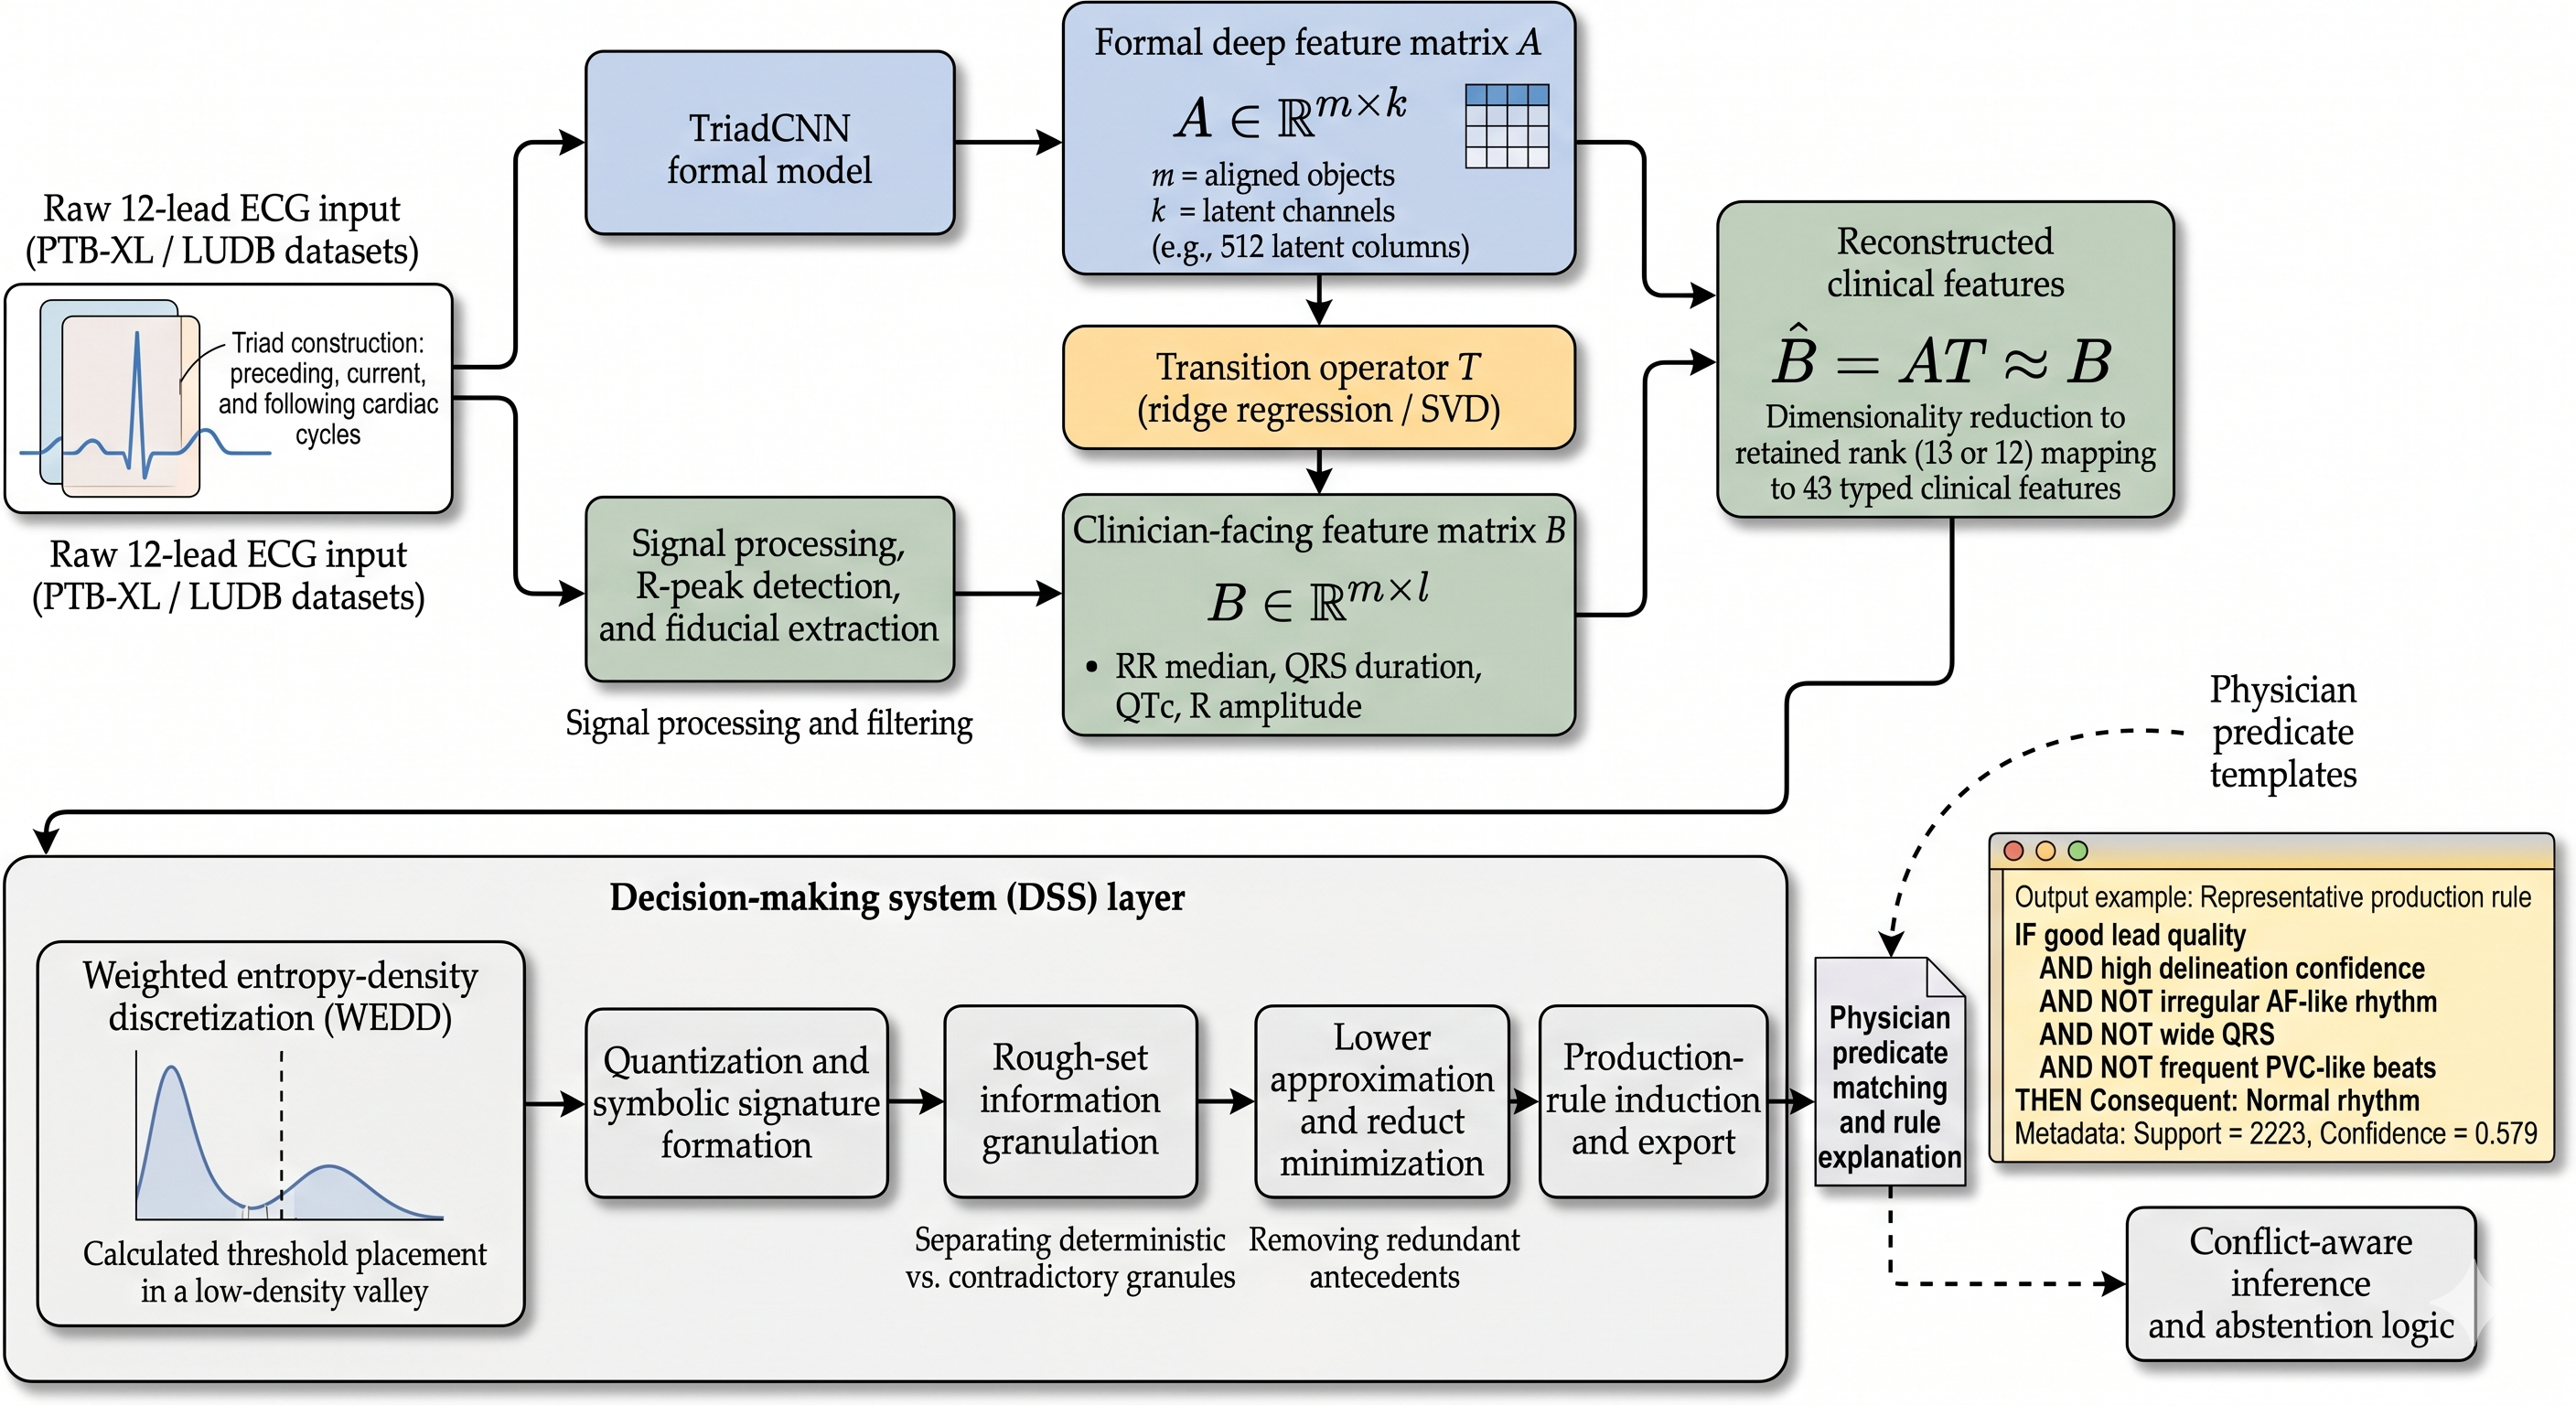
\includegraphics[width=\linewidth,height=0.77\textheight,keepaspectratio]{assets_ecg/87_fig_1.png}
  \slidecaption{\textbf{Fig. 1.} End-to-end ECG audit workflow linking latent neural encoding,
  semantic transition, WEDD discretization, rough-set granulation, and conflict-aware inference.}

  \column{0.24\textwidth}
  \begin{block}{Decision system}
  \small
  \[
    S=(U,C,d,V,f).
    \tag{1}
  \]
  \end{block}
  {\scriptsize
  $U$: ECG objects; $C$: semantic attributes; $d$: decision; $V$: domains;
  $f$: object--attribute information.
  \par}
  \vspace{0.35em}
  \begin{exampleblock}{Separation}
  \scriptsize
  Frozen prediction; independently inspectable explanation.
  \end{exampleblock}
\end{columns}
\end{frame}

% 5 -----------------------------------------------
\begin{frame}{Global Semantic Transition}
\small
\begin{columns}[T,onlytextwidth]
  \column{0.58\textwidth}
  \begin{beamercolorbox}[wd=\linewidth,sep=0.55em]{equation box}
  {\small
  \[
    \widehat{B}=AT\approx B .
    \tag{2}
  \]
  \[
    T_{\lambda}=\arg\min_T
    \left\lVert A_{\mathrm{red}}T-B_{\mathrm{fit}}\right\rVert_F^2
    +\lambda\lVert T\rVert_F^2 .
    \tag{3}
  \]
  \[
    T_{\lambda}=
    \left(A_{\mathrm{red}}^{\top}A_{\mathrm{red}}+\lambda I\right)^{-1}
    A_{\mathrm{red}}^{\top}B_{\mathrm{fit}} .
    \tag{4}
  \]
  \par}
  \end{beamercolorbox}

  \column{0.38\textwidth}
  \begin{block}{Inputs}
  \scriptsize
  \begin{itemize}\compactitem
    \item $A$: aligned latent features.
    \item $B$: clinical feature targets.
    \item $\lambda$: Tikhonov regularization.
  \end{itemize}
  \end{block}
  \begin{exampleblock}{Audit property}
  \scriptsize
  Every coefficient links latent evidence to a named clinical measurement;
  no second opaque model.
  \end{exampleblock}
  \vspace{0.15em}
  \metric{512 latent columns $\rightarrow$ 43 clinical targets}
\end{columns}
\end{frame}

% 6 -----------------------------------------------
\begin{frame}{Weighted Entropy-Density Discretization}
\scriptsize
\begin{columns}[T,onlytextwidth]
  \column{0.49\textwidth}
  \begin{beamercolorbox}[wd=\linewidth,sep=0.42em]{equation box}
  {\scriptsize
  \[
  \begin{aligned}
  U_j^{-}(t)&=\{x_i\in U:f(x_i,c_j)\le t\},\\[-0.1em]
  U_j^{+}(t)&=\{x_i\in U:f(x_i,c_j)>t\}.
  \end{aligned}
  \tag{5}
  \]
  \[
  H_d(W)=-\sum_{y\in V_d}p_W(y)\log p_W(y).
  \tag{6}
  \]
  \[
  H_j(t)=\frac{|U_j^-|}{|U|}H_d(U_j^-)
  +\frac{|U_j^+|}{|U|}H_d(U_j^+).
  \tag{7}
  \]
  \par}
  \end{beamercolorbox}
  \vspace{0.35em}
  \begin{block}{Entropy term}
  \small
  Candidate thresholds should separate decision labels, not merely partition
  the numeric range.
  \end{block}

  \column{0.49\textwidth}
  \begin{beamercolorbox}[wd=\linewidth,sep=0.42em]{equation box}
  {\scriptsize
  \[
  \begin{aligned}
  J_j(t)&=\alpha H_j(t)+(1-\alpha)p_j(t),\\[-0.1em]
  t_j^\ast&=\arg\min_{t\in\Theta_j}J_j(t).
  \end{aligned}
  \tag{8}
  \]
  \[
  q_j(z)=r\ \text{if}\ \tau_{j,r}<z\le\tau_{j,r+1},\qquad
  \sigma(x_i)=(q_1,\ldots,q_l).
  \tag{9}
  \]
  \par}
  \end{beamercolorbox}
  \vspace{0.35em}
  \begin{exampleblock}{Density term}
  \small
  WEDD favors low-density valleys, reducing symbolic state changes under
  small semantic perturbations.
  \end{exampleblock}
  \metric{Continuous measurements $\rightarrow$ stable symbolic states}
\end{columns}
\end{frame}

% 7 -----------------------------------------------
\begin{frame}{Rough-Set Granulation and Rule Export}
\scriptsize
\centering
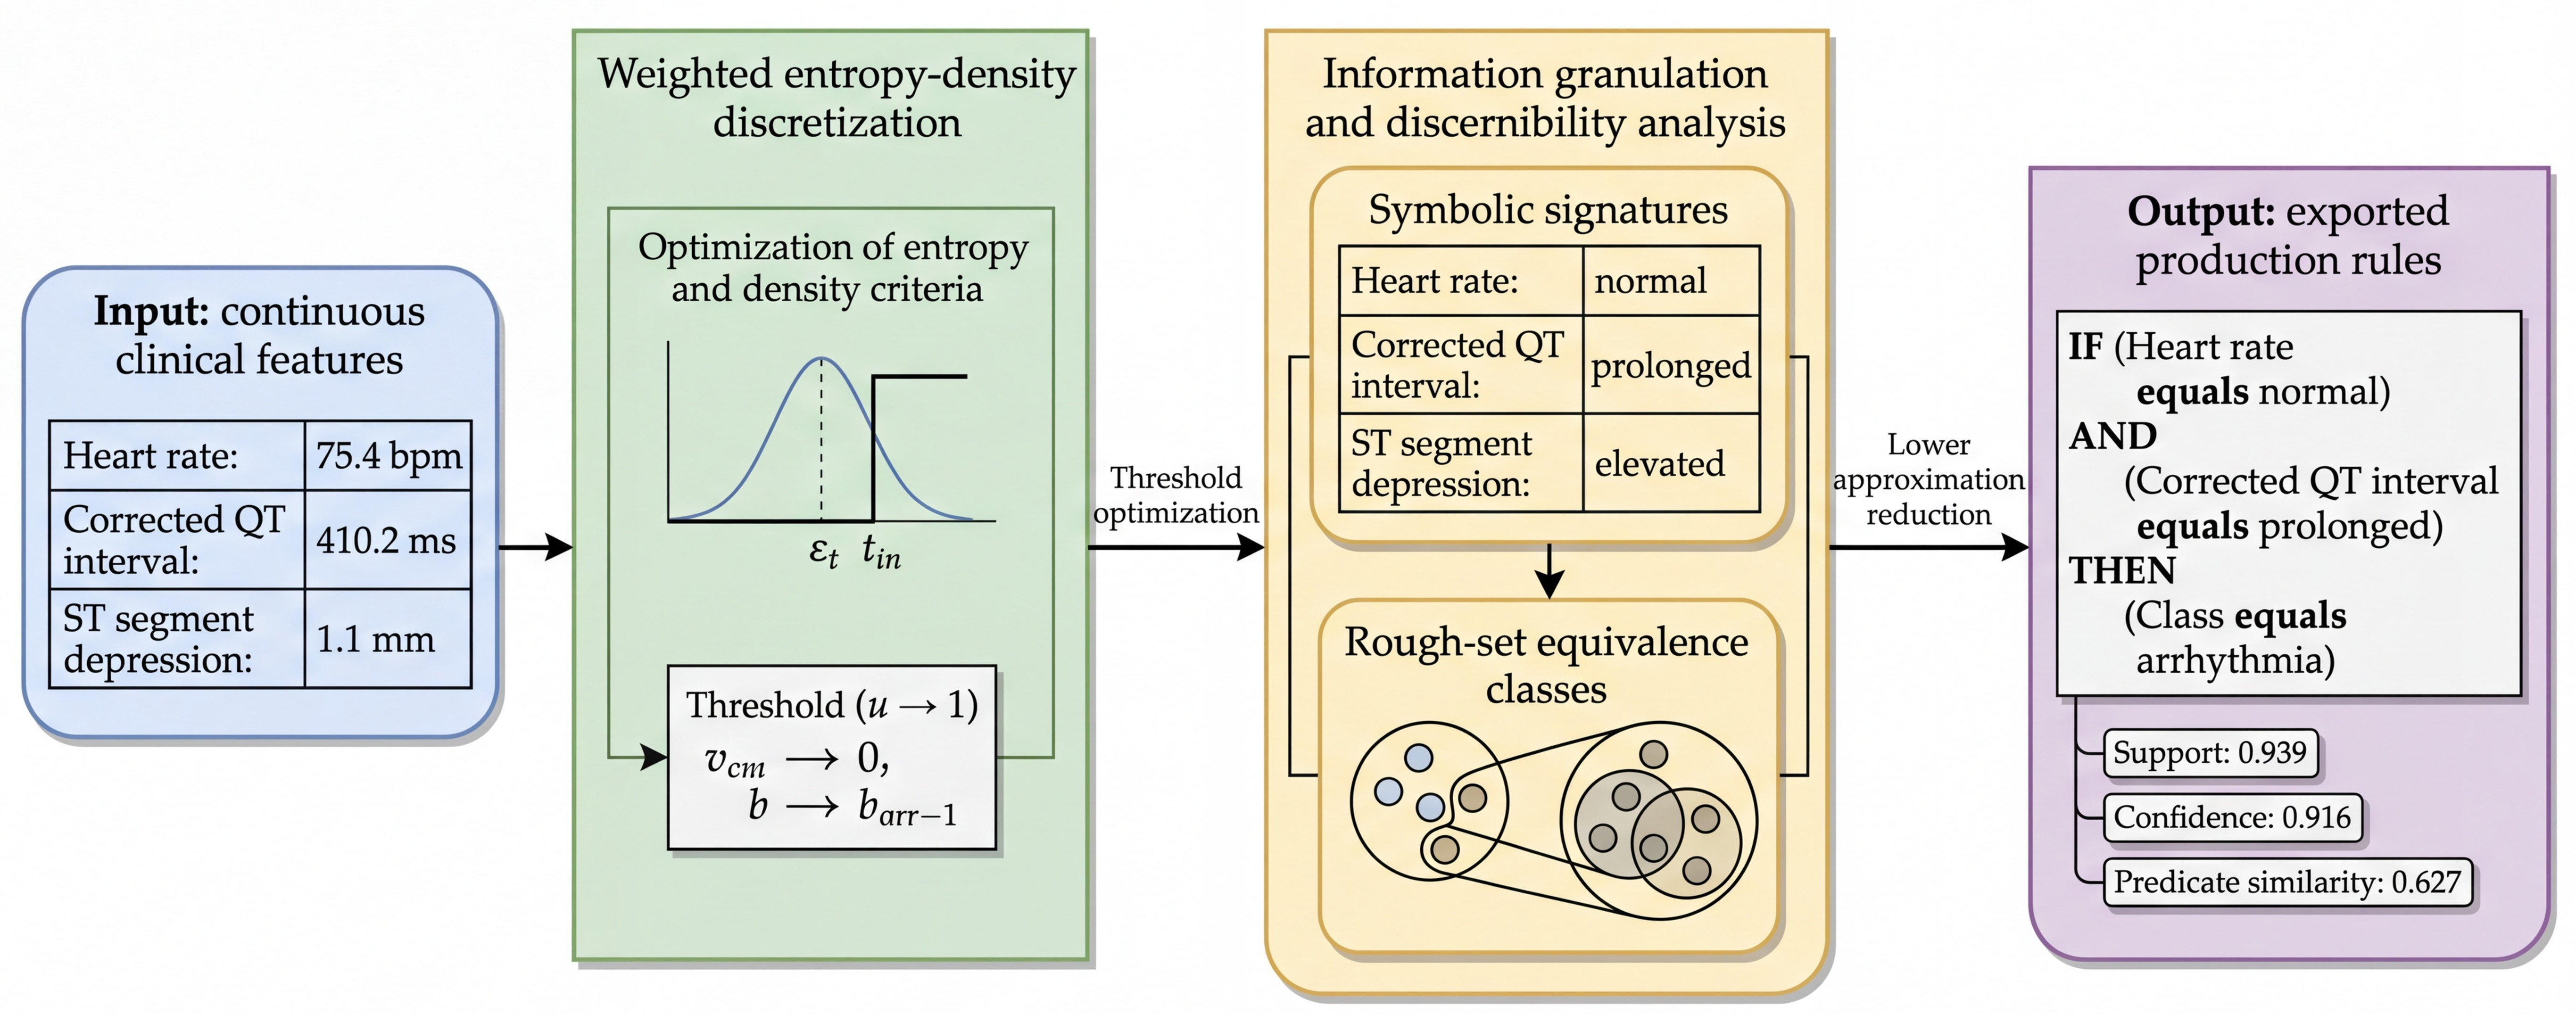
\includegraphics[width=\linewidth,height=0.49\textheight,keepaspectratio]{assets_ecg/87_fig_2.jpg}
\slidecaption{\textbf{Fig. 2.} Detailed rule-extraction logic using symbolic signatures, discernibility analysis, and rule export.}
\vspace{0.15em}
\begin{columns}[T,onlytextwidth]
  \column{0.34\textwidth}
  \begin{beamercolorbox}[wd=\linewidth,sep=0.28em]{equation box}
  {\scriptsize
  \begin{equation*}
  \resizebox{0.76\linewidth}{!}{$\displaystyle
  \mathrm{IND}(P)=\{(x_i,x_r)\in U^2:\forall c_j\in P,\,
  f(x_i,c_j)=f(x_r,c_j)\}.$}
  \tag{10}
  \end{equation*}
  \par}
  \end{beamercolorbox}

  \column{0.29\textwidth}
  \begin{beamercolorbox}[wd=\linewidth,sep=0.28em]{equation box}
  {\scriptsize
  \[
  \underline{P}(Y)=\{x\in U:[x]_P\subseteq Y\}.
  \tag{11}
  \]
  \par}
  \end{beamercolorbox}

  \column{0.33\textwidth}
  \begin{beamercolorbox}[wd=\linewidth,sep=0.28em]{equation box}
  {\scriptsize
  \[
  r:\bigcap_{c_j\in P}(c_j=s_j)\Rightarrow d=y_r .
  \tag{12}
  \]
  \par}
  \end{beamercolorbox}
\end{columns}
\vspace{0.05em}
{\scriptsize
Only pure lower-approximation granules become deterministic rules; boundary
objects remain visible as uncertainty evidence.
\par}
\end{frame}

% 8 -----------------------------------------------
\begin{frame}{Audit Metrics, Fallback, and Alignment}
\scriptsize
\begin{columns}[T,onlytextwidth]
  \column{0.49\textwidth}
  \begin{beamercolorbox}[wd=\linewidth,sep=0.34em]{equation box}
  {\scriptsize
  \[
  \begin{aligned}
  \mathrm{supp}(r)&=|\{x\in U:x\models\mathrm{ante}(r)\}|,\\[-0.1em]
  \mathrm{conf}(r)&=
  \frac{|\{x:x\models\mathrm{ante}(r),d(x)=y_r\}|}{\mathrm{supp}(r)}.
  \end{aligned}
  \tag{13}
  \]
  \[
  \mathrm{Cov}=\frac{|\{x\in U:R(x)\ne\varnothing\}|}{|U|}.
  \tag{14}
  \]
  \[
  E_{\mathrm{MAE}}=\frac{1}{ml}\sum_i\sum_j
  \left|B_{\mathrm{fit},ij}-\widehat{B}_{\mathrm{fit},ij}\right|.
  \tag{15}
  \]
  \par}
  \end{beamercolorbox}

  \column{0.49\textwidth}
  \begin{beamercolorbox}[wd=\linewidth,sep=0.34em]{equation box}
  {\scriptsize
  \[
  \mathrm{CR}=
  \frac{|\{x\in U:|R_{\mathrm{conflicting}}(x)|>1\}|}{|U|}.
  \tag{16}
  \]
  \[
  d_H(\sigma(x_i),\sigma(x_r))=
  \sum_j\mathbf{1}\{\sigma_j(x_i)\ne\sigma_j(x_r)\}.
  \tag{17}
  \]
  \[
  \scalebox{0.88}{$\displaystyle
  S(r,P)=w_fS_f+w_vS_v+w_lS_l+w_cS_c+w_dS_d
  -\lambda_{\mathrm{safe}}^2\Omega(r,P).$}
  \tag{18}
  \]
  \par}
  \end{beamercolorbox}
\end{columns}
\vspace{0.15em}
\begin{columns}[T,onlytextwidth]
  \column{0.49\textwidth}
  \begin{block}{Exact audit}
  \scriptsize
  Coverage, support, confidence, reconstruction error, and conflict are
  directly measurable.
  \end{block}
  \column{0.49\textwidth}
  \begin{exampleblock}{Transparent fallback}
  \scriptsize
  Hamming distance and physician-template alignment remain separate from the
  frozen classifier's uncertainty.
  \end{exampleblock}
\end{columns}
\end{frame}

\section{Experiments}

% 9 -----------------------------------------------
\begin{frame}{Benchmarks and Reconstruction Protocol}
\scriptsize
\begin{columns}[T,onlytextwidth]
  \column{0.49\textwidth}
  {\scriptsize\textbf{Table 1.} Benchmark feature artifacts used for semantic
  reconstruction and rule induction.\par}
  \vspace{0.12em}
  \resizebox{\linewidth}{!}{%
  \begin{tabular}{llrrr}
  \toprule
  \textbf{Branch} & \textbf{Split} & \textbf{Rows} &
  \textbf{Feature cols.} & \textbf{Null rate}\\
  \midrule
  B1 (PTB-XL) & train & 10,000 & 49 & 0.1131\\
  B1 (PTB-XL) & validation & 2183 & 49 & 0.1134\\
  B1 (PTB-XL) & test & 2198 & 49 & 0.1134\\
  B2 (LUDB) & train & 120 & 49 & 0.1151\\
  B2 (LUDB) & validation & 40 & 49 & 0.1143\\
  B2 (LUDB) & test & 40 & 49 & 0.1179\\
  \bottomrule
  \end{tabular}}

  \column{0.49\textwidth}
  {\scriptsize\textbf{Table 2.} Transition-operator metadata and
  explanation-quality estimates.\par}
  \vspace{0.12em}
  \resizebox{\linewidth}{!}{%
  \begin{tabular}{lrrrrll}
  \toprule
  \textbf{Branch} & \textbf{Latent} & \textbf{Rank} & \textbf{Targets} &
  \textbf{Split} & \textbf{MAE} & \textbf{95\% CI}\\
  \midrule
  B1 & 512 & 13 & 43 & val. & 0.4048 & [0.4010, 0.4089]\\
  B1 & 512 & 13 & 43 & test & 0.4032 & [0.3996, 0.4069]\\
  B2 & 512 & 12 & 43 & val. & 0.4564 & [0.4198, 0.4923]\\
  B2 & 512 & 12 & 43 & test & 0.3722 & [0.3490, 0.3939]\\
  \bottomrule
  \end{tabular}}
\end{columns}
\vspace{2.5em}
\begin{columns}[T,onlytextwidth]
  \column{0.31\textwidth}\metric{PTB-XL: 10,000 rule objects}
  \column{0.31\textwidth}\metric{LUDB: morphology validation}
  \column{0.31\textwidth}\metric{Five-seed bootstrap estimates}
\end{columns}
\vspace{0.32em}
{\small
B1 validation/test MAE differs by only $0.0016$; B2's wider validation
interval reflects its 40-object split.
\par}
\end{frame}

\section{Results}

% 10 ----------------------------------------------
\begin{frame}{Semantic Reconstruction Diagnostics}
\small
\begin{columns}[T,onlytextwidth]
  \column{0.49\textwidth}
  \centering
  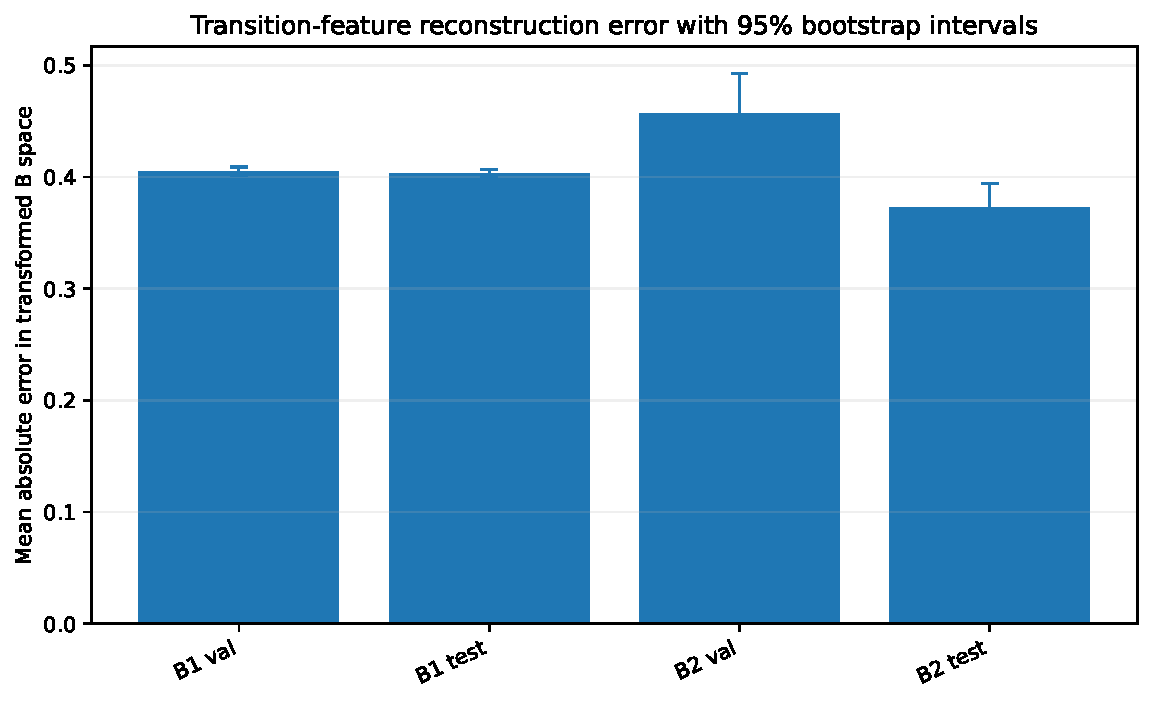
\includegraphics[width=\linewidth,height=0.60\textheight,keepaspectratio]{assets_ecg/87_fig_3_explanation_mae_ci.pdf}
  \slidecaption{\textbf{Fig. 3.} Explanation-layer reconstruction MAE with 95\%
  bootstrap intervals for B1 and B2 validation/test splits.}

  \column{0.49\textwidth}
  \centering
  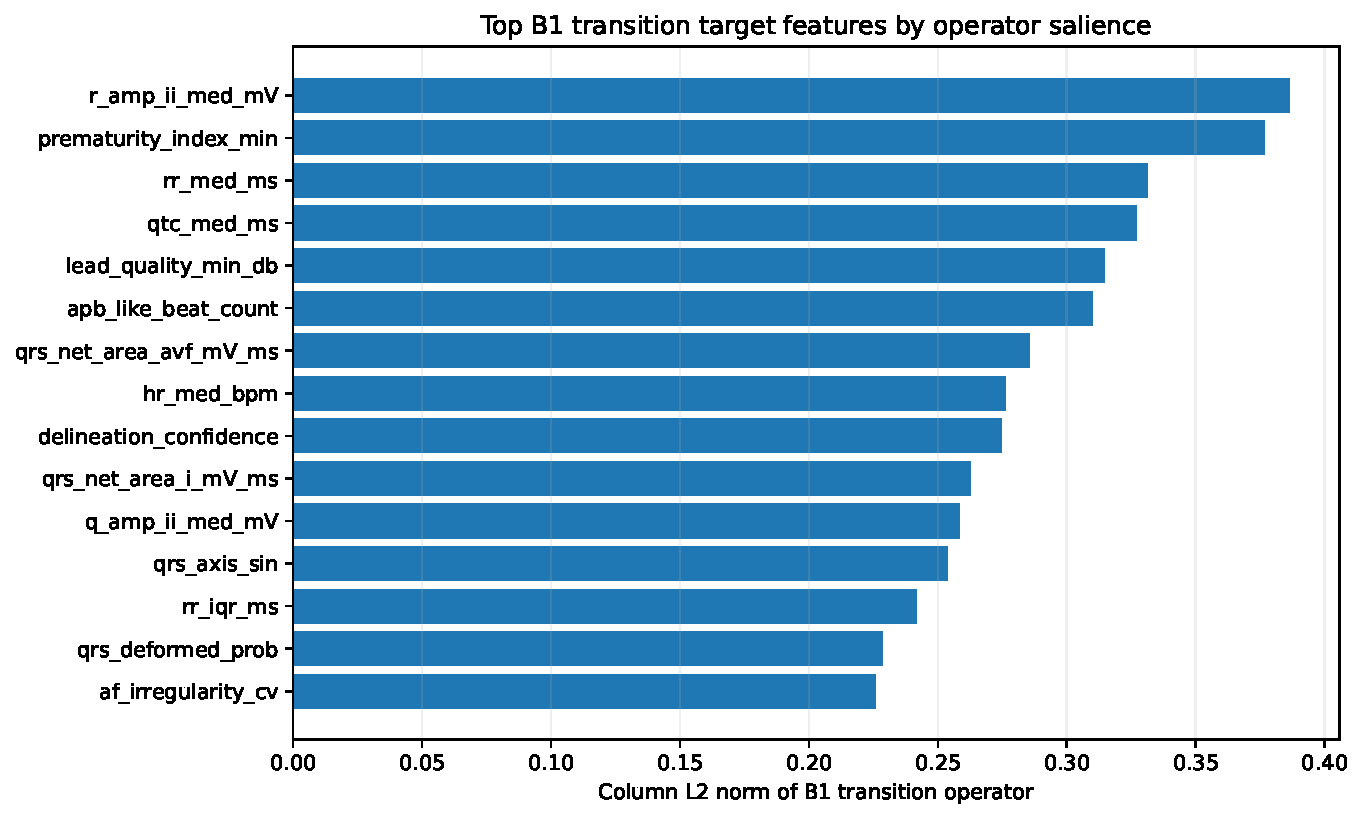
\includegraphics[width=\linewidth,height=0.60\textheight,keepaspectratio]{assets_ecg/87_fig_4_b1_transition_salience.pdf}
  \slidecaption{\textbf{Fig. 4.} B1 transition-feature salience measured by the
  $L_2$ norm of fitted transition weights for clinical target features.}
\end{columns}
\vspace{0.10em}
\begin{beamercolorbox}[wd=\linewidth,sep=0.45em]{metric box}
{\small\centering
Stable reconstruction coexists with clinically legible salience:
R-amplitude, prematurity, RR behavior, QTc, and lead quality dominate.
\par}
\end{beamercolorbox}
\end{frame}

% 11 ----------------------------------------------
\begin{frame}{Rulebook Coverage, Conflict, and Support}
\scriptsize
{\scriptsize\textbf{Table 3.} Rulebook coverage, conflict, and abstention behavior.\par}
\vspace{0.1em}
\begin{tabularx}{\linewidth}{lrrrrrrY}
\toprule
\textbf{Branch} & \textbf{Universe} & \textbf{Features} & \textbf{Rules} &
\textbf{Coverage} & \textbf{Abstention} & \textbf{Conflict} & \textbf{Labels}\\
\midrule
B1 & 10,000 & 24 & 8 & 0.939 & 0.061 & 0.0707 &
AF; AFL; APB; LBBB; Normal; Other; PVC; RBBB\\
B2 & 120 & 4 & 2 & 0.900 & 0.100 & 0.0000 & Other/unmapped\\
\bottomrule
\end{tabularx}
\vspace{0.18em}
\begin{columns}[T,onlytextwidth]
  \column{0.67\textwidth}
  \centering
  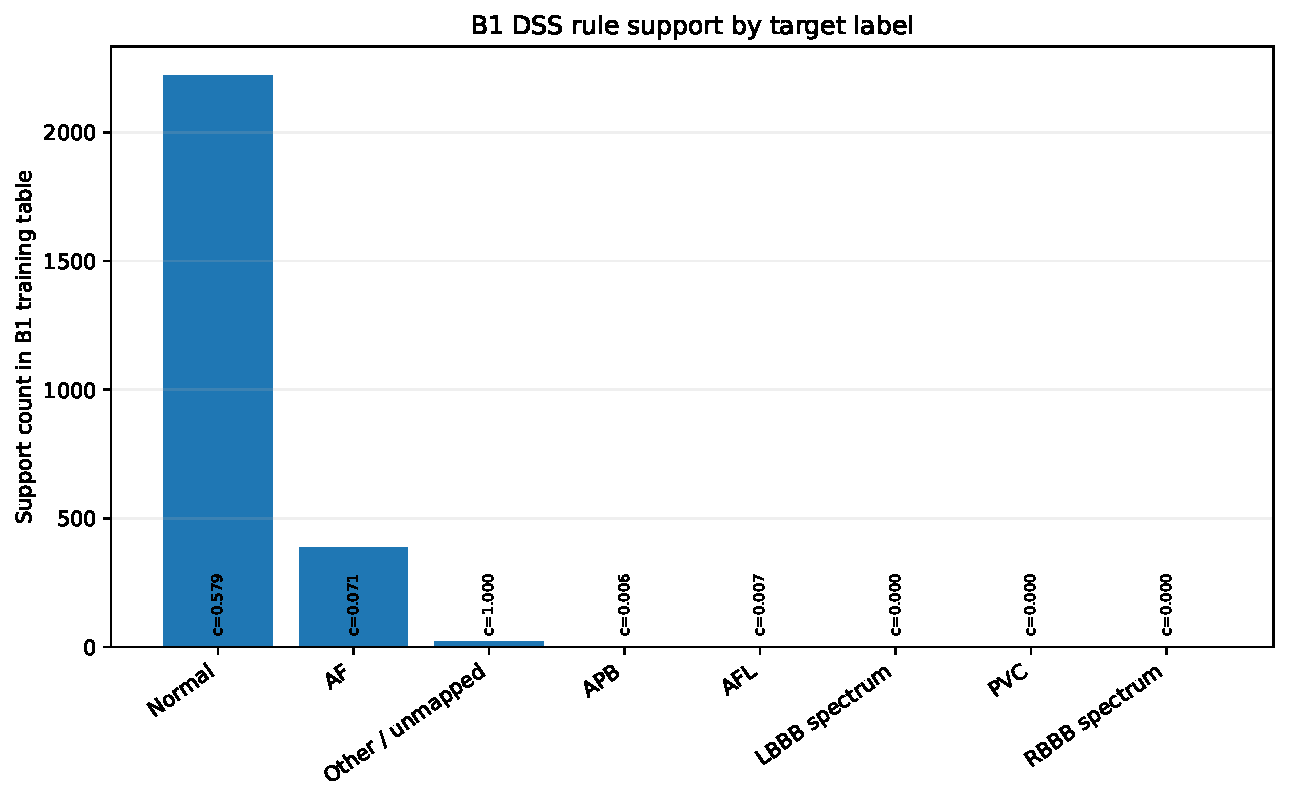
\includegraphics[width=\linewidth,height=0.48\textheight,keepaspectratio]{assets_ecg/87_fig_5_b1_rule_support.pdf}
  \slidecaption{\textbf{Fig. 5.} Support counts for B1 production rules; zero-support template predicates are retained as alignment artifacts.}

  \column{0.29\textwidth}
  \begin{exampleblock}{B1 audit profile}
  \small
  \textbf{Coverage:} 93.9\%\\[0.2em]
  \textbf{Conflict:} 7.07\%\\[0.2em]
  \textbf{Abstention:} 6.1\%\\[0.35em]
  {\scriptsize\textbf{Reading:} Normal carries the largest empirical
  support; zero-support templates remain explicit.\par}
  \end{exampleblock}
\end{columns}
\end{frame}

% 12 ----------------------------------------------
\begin{frame}{Exported Rules and Predicate Alignment}
\scriptsize
{\scriptsize\textbf{Table 4.} Representative exported rules and
predicate-level audit evidence.\par}
\vspace{0.08em}
{\scriptsize
\begingroup
\fontsize{6.3}{6.8}\selectfont
\setlength{\tabcolsep}{1.7pt}
\renewcommand{\arraystretch}{0.96}
\begin{tabularx}{\linewidth}{@{}p{0.9cm}p{1.35cm}rrY@{}}
\toprule
\textbf{Branch} & \textbf{Consequent} & \textbf{Support} &
\textbf{Conf.} & \textbf{Antecedent summary}\\
\midrule
B1 & AF & 388 & 0.071 & AF irregularity present; not paced-like; no f-wave-present ratio.\\
B1 & Normal & 2223 & 0.579 & Good quality; high delineation confidence; not AF-like; not wide QRS; not PVC-like.\\
B1 & Other & 20 & 1.000 & Regular AF-irregularity state; good quality; deformed QRS; normal QTc; V1 r-prime absent; ST V5 depressed.\\
B2 & Other & 82 & 1.000 & Lead quality is good.\\
B2 & Other & 26 & 1.000 & Lead quality is marginal.\\
\bottomrule
\end{tabularx}
\endgroup
\par}
\vspace{0.18em}
{\scriptsize\textbf{Table 5.} Physician-predicate alignment summary for
exported benchmark rules.\par}
\vspace{0.08em}
{\scriptsize
\begingroup
%\fontsize{6.3}{6.8}\selectfont
\setlength{\tabcolsep}{1.7pt}
\renewcommand{\arraystretch}{0.96}
\begin{tabularx}{\linewidth}{@{}p{0.9cm}p{2.25cm}p{2.3cm}Y@{}}
\toprule
\textbf{Branch} & \textbf{Rule group} & \textbf{Similarity evidence} &
\textbf{Interpretation}\\
\midrule
B1 & Structured morphology & upper range near 0.6273 &
Best alignment for bundle-branch patterns with tight feature clusters.\\
B1 & Rhythm and normal templates & lower range near 0.5245 &
Lower alignment because rhythm interpretation depends on temporal context and label mapping.\\
B2 & Lead-quality routing & 0.6090 &
Moderate alignment for quality-oriented semantic predicates.\\
\bottomrule
\end{tabularx}
\endgroup
\par}
\end{frame}

% 13 ----------------------------------------------
\begin{frame}{Classifier-Linked Audit}
\scriptsize
{\scriptsize\textbf{Table 7.} Held-out PTB-XL classifier-linked explanation behavior.\par}
\vspace{0.08em}
\begin{tabularx}{\linewidth}{lrrrrrr}
\toprule
\textbf{Group} & \textbf{$n$} & \textbf{Coverage} & \textbf{Abstain} &
\textbf{Conflict} & \textbf{Rule--head agreement} & \textbf{Margin}\\
\midrule
All & 2198 & 0.9950 & 0.0050 & 0.0073 & 0.2332 & 0.5791\\
Correct & 1546 & 0.9955 & 0.0045 & 0.0084 & 0.2664 & 0.6461\\
Error & 652 & 0.9939 & 0.0061 & 0.0046 & 0.1543 & 0.4204\\
\bottomrule
\end{tabularx}
\vspace{0.28em}
{\scriptsize\textbf{Table 8.} Selective audit-routing performance on the
held-out PTB-XL test split.\par}
\vspace{0.08em}
\begin{tabularx}{\linewidth}{Yrrrrrr}
\toprule
\textbf{Policy} & \textbf{Retained $n$} & \textbf{Coverage} &
\textbf{Accuracy} & \textbf{Flagged error} & \textbf{Failure OR} & \textbf{$p$}\\
\midrule
No rejection & 2198 & 1.0000 & 0.7034 & -- & -- & --\\
Reject rule flags & 2171 & 0.9877 & 0.7029 & 0.2593 & Not enriched & $>0.05$\\
Margin $<0.1554$ & 1977 & 0.8995 & 0.7395 & 0.6199 & 4.63 & $<0.001$\\
\bottomrule
\end{tabularx}
\vspace{0.26em}
\begin{columns}[T,onlytextwidth]
  \column{0.48\textwidth}
  \begin{beamercolorbox}[wd=\linewidth,sep=0.45em]{block body alerted}
  {\scriptsize\textbf{Do not conflate signals.} Rule conflict and abstention
  encode structural ambiguity, not calibrated classifier error.\par}
  \end{beamercolorbox}
  \column{0.48\textwidth}
  \begin{beamercolorbox}[wd=\linewidth,sep=0.45em]{block body example}
  {\scriptsize\textbf{Selective routing works.} The validation-locked margin
  raises retained accuracy from 0.7034 to 0.7395 at 0.8995 coverage.\par}
  \end{beamercolorbox}
\end{columns}
\end{frame}

\section{Discussion}

% 14 ----------------------------------------------
\begin{frame}{Evidence Synthesis and Outlook}
\small
\begin{columns}[T,onlytextwidth]
  \column{0.30\textwidth}
  \begin{exampleblock}{Evidence supports}
  \scriptsize
  \begin{itemize}\compactitem
    \item Stable B1 reconstruction.
    \item 93.9\% rule coverage.
    \item Explicit uncertainty logs.
    \item Coverage independent of correctness.
  \end{itemize}
  \end{exampleblock}

  \column{0.30\textwidth}
  \begin{alertblock}{Current limits}
  \scriptsize
  \begin{itemize}\compactitem
    \item Global linear transition.
    \item Threshold-sensitive discretization.
    \item Small LUDB branch.
    \item Template score is not physician agreement.
  \end{itemize}
  \end{alertblock}

  \column{0.30\textwidth}
  \begin{block}{Next validation}
  \scriptsize
  \begin{itemize}\compactitem
    \item Prospective physician annotations.
    \item External cohort shift tests.
    \item Dynamic feature dictionaries.
    \item Joint fidelity--logic optimization.
  \end{itemize}
  \end{block}
\end{columns}
\vspace{0.18em}
\begin{beamercolorbox}[wd=0.97\linewidth,sep=0.55em]{metric box}
{\small\centering\bfseries
Main conclusion: a frozen ECG classifier can gain an auditable semantic
rulebook without retraining, while unresolved cases remain visible.
\par}
\end{beamercolorbox}
\vfill
{\scriptsize
\textbf{Acknowledgments.} PhysioNet, PTB-XL, and LUDB maintainers.
\par}
\end{frame}

% 15 ----------------------------------------------
\begin{frame}{Contact}
\scriptsize
\begin{columns}[T,onlytextwidth]
  \column{0.47\textwidth}
  \begin{block}{Authors and correspondence}
  \scriptsize
  \textbf{Pavlo Radiuk}\textsuperscript{1}\\
  \href{mailto:radiukp@khmnu.edu.ua}{radiukp@khmnu.edu.ua}\\[0.25em]
  \vspace{0.35em}
  \textbf{Oleksander Barmak}\textsuperscript{1}\\
  \href{mailto:barmako@khmnu.edu.ua}{barmako@khmnu.edu.ua}\\[0.25em]
  \vspace{0.35em}
  \textbf{Iurii Krak}\textsuperscript{2,3}\\
  \href{mailto:iurii.krak@knu.ua}{iurii.krak@knu.ua}
  \end{block}

  \column{0.49\textwidth}
  \begin{block}{Affiliations}
  \scriptsize
  \textsuperscript{1}Khmelnytskyi National University\\[0.35em]
  \textsuperscript{2}Taras Shevchenko National University of Kyiv\\[0.35em]
  \textsuperscript{3}V.M. Glushkov Institute of Cybernetics
  \end{block}
  \begin{exampleblock}{Discussion prompt}
  \scriptsize
  Which clinical predicates should be prioritized in the next prospective
  audit study?
  \end{exampleblock}
\end{columns}
\vfill
{\scriptsize\centering Supporting organizations and supplied project identities\par}
\vspace{0.18em}
\begin{center}
  \supportlogos
\end{center}
\end{frame}

\end{document}
